\documentclass[]{article}


\usepackage{float}
\usepackage[italian]{babel}

% Set page size and margins
% Replace `letterpaper' with`a4paper' for UK/EU standard size
\usepackage[letterpaper,top=3cm,bottom=3cm,left=3cm,right=3cm,marginparwidth=1.75cm]{geometry}

% Useful packages
\usepackage{amsmath}
\usepackage{graphicx}
\usepackage[colorlinks=true, allcolors=blue]{hyperref}


\title{SMSecure - Documentazione}
\author{Samuele Russo   matr.0512113317}


\begin{document}
\maketitle

\newpage

\tableofcontents

\newpage

\section{Introduzione}

    L'aumento esponenziale dell'utilizzo di dispositivi mobili ha reso gli SMS uno dei principali canali di comunicazione. Tuttavia, insieme a questa crescita, si è verificato un forte incremento del numero di spam SMS; ovvero messaggi caratterizzati da contenuti promozionali non richiesti, pubblicità ingannevoli o addirittura truffe; compromettendo l'efficienza e la sicurezza delle comunicazioni personali e professionali.\\
    Tutto il codice, il modello, la presentazione nonchè tale documentazione, si possono trovare presso tale repository \href{https://github.com/russosamuele/SMSecure.git}{GitHub}


    \subsection{Obiettivi}

        Tale progetto di Fondamenti di Intelligenza Artificiale, il mio primo approccio in questo ambito, si propone di sviluppare un filtro anti-spam sms per migliorare l'esperienza degli utenti nel gestire i propri messaggi. Ho scelto tale tematica perchè relativamente semplice, e quindi in grado di farmi apprendere il più possibile le basi del Machine Learning.

        Gli obiettivi principali includono:
        \begin{itemize}
            \item l'analisi approfondita di grandi quantità di SMS        estrapolati da un dataset.
            \item l'identificazione di feature associate ai               messaggi indesiderati.
            \item l'implementazione di un modello di apprendimento in grado di classificare in modo affidabile messagi spam e legittimi.
        \end{itemize}

    \subsection{Specifica PEAS}
        \begin{itemize}
            \item Performance (misure di prestazione adottate per valutare l’operato di un agente), nel mio caso verranno valutate la precisione di classificazione e l'accuratezza. Inoltre sarà anche considerato il tasso di falsi positivi, ovvero messaggi legittimi che vengono erroneamente etichettati come spam.
            \item Environment (elementi che formano l’ambiente), nel mio caso sarà costituito dal flusso di messaggi ricevuti. '\textit{maggiori dettagli in sezione 1.3}'
            \item Actuators (attuatori disponibili all’agente per intraprendere le azioni), nel mio caso sarà la capacità del sistema di etichettare i messaggi in arrivo come spam o ham.
            \item Sensors (sensori attraverso i quali l'agente riceve gli input percettivi), nel mio caso l'agente va ad acquisire i dati utili per classificare un messaggio, incluso il contenuto del messaggio, ma anche eventuali feature costruite (numero di parole ecc.)
        \end{itemize}

        \subsection{Caratteristiche dell'ambiente}
            L'ambiente è:
            \begin{itemize}
                \item Parzialmente osservabile, in quanto non si ha accesso alle informazioni del mittente.
                \item Stocastico, infatti i messaggi inviati dagli utenti sono influenzati da fattori non prevedibili.
                \item Singolo agente.
                \item Dinamico, difatti potrebbero venire a crearsi nuovi schemi di messaggi spam.
                \item Discreto, in quanto non sono presenti variabili continue (ad esempio la frequenza di invio di un determinato mittente, ma io non ho trovato tale informazioni).
                \item Sequenziale, difatti il filtro anti-spam verrà pienamente influenzato dalle esperienze passate, per andare a prendere delle decisioni.
            \end{itemize}

        \subsection{Analisi del problema}
            Quindi in poche parole SMSecure mira a costruire un filtro anti-spam sms, si tratta quindi di un problema di Machine Learning, più nello specifico di un problema di apprendimento supervisionato, nonchè di classificazione. Nelle successive sezioni vado a descrivere tutte le problematiche che ho affrontato: dalla scelta dei dati, fino al deploy del modello.\\
            Per quanto riguarda le tecnologie che ho utilizzato per lo sviluppo del progetto, abbiamo:
            \begin{itemize}
                \item Python (in dettaglio le librerie per ML, come sickitLearn, Pandas,  ecc.),
                \item JupyterNotebook all'interno dell'IDE PyCharm
                \item GitHub per il versionamento,
                \item Overleaf e Canva per documentazione e presentazione.
            \end{itemize}
\newpage
\section{Data Understanding}
    Tale fase è composta da più punti:
    \begin{itemize}
        \item Acquisizione dei dati
        \item Esplorazione dei dati
        \item Analisi della qualità dei dati
    \end{itemize}
    \subsection{Acquisizione dei dati}
        L'acquisizione dei dati è il processo di raccolta, ed organizzazione dei dati necessari per andare a creare un modello di ML. Con gli obiettivi chiari e definiti, sono andato alla ricerca di un dataset sul web, fino a trovarne uno molto interessante su Kaggle; una piattaforma, nonchè comunità online di data science. \\

        \begin{figure}[H]
            \centering
            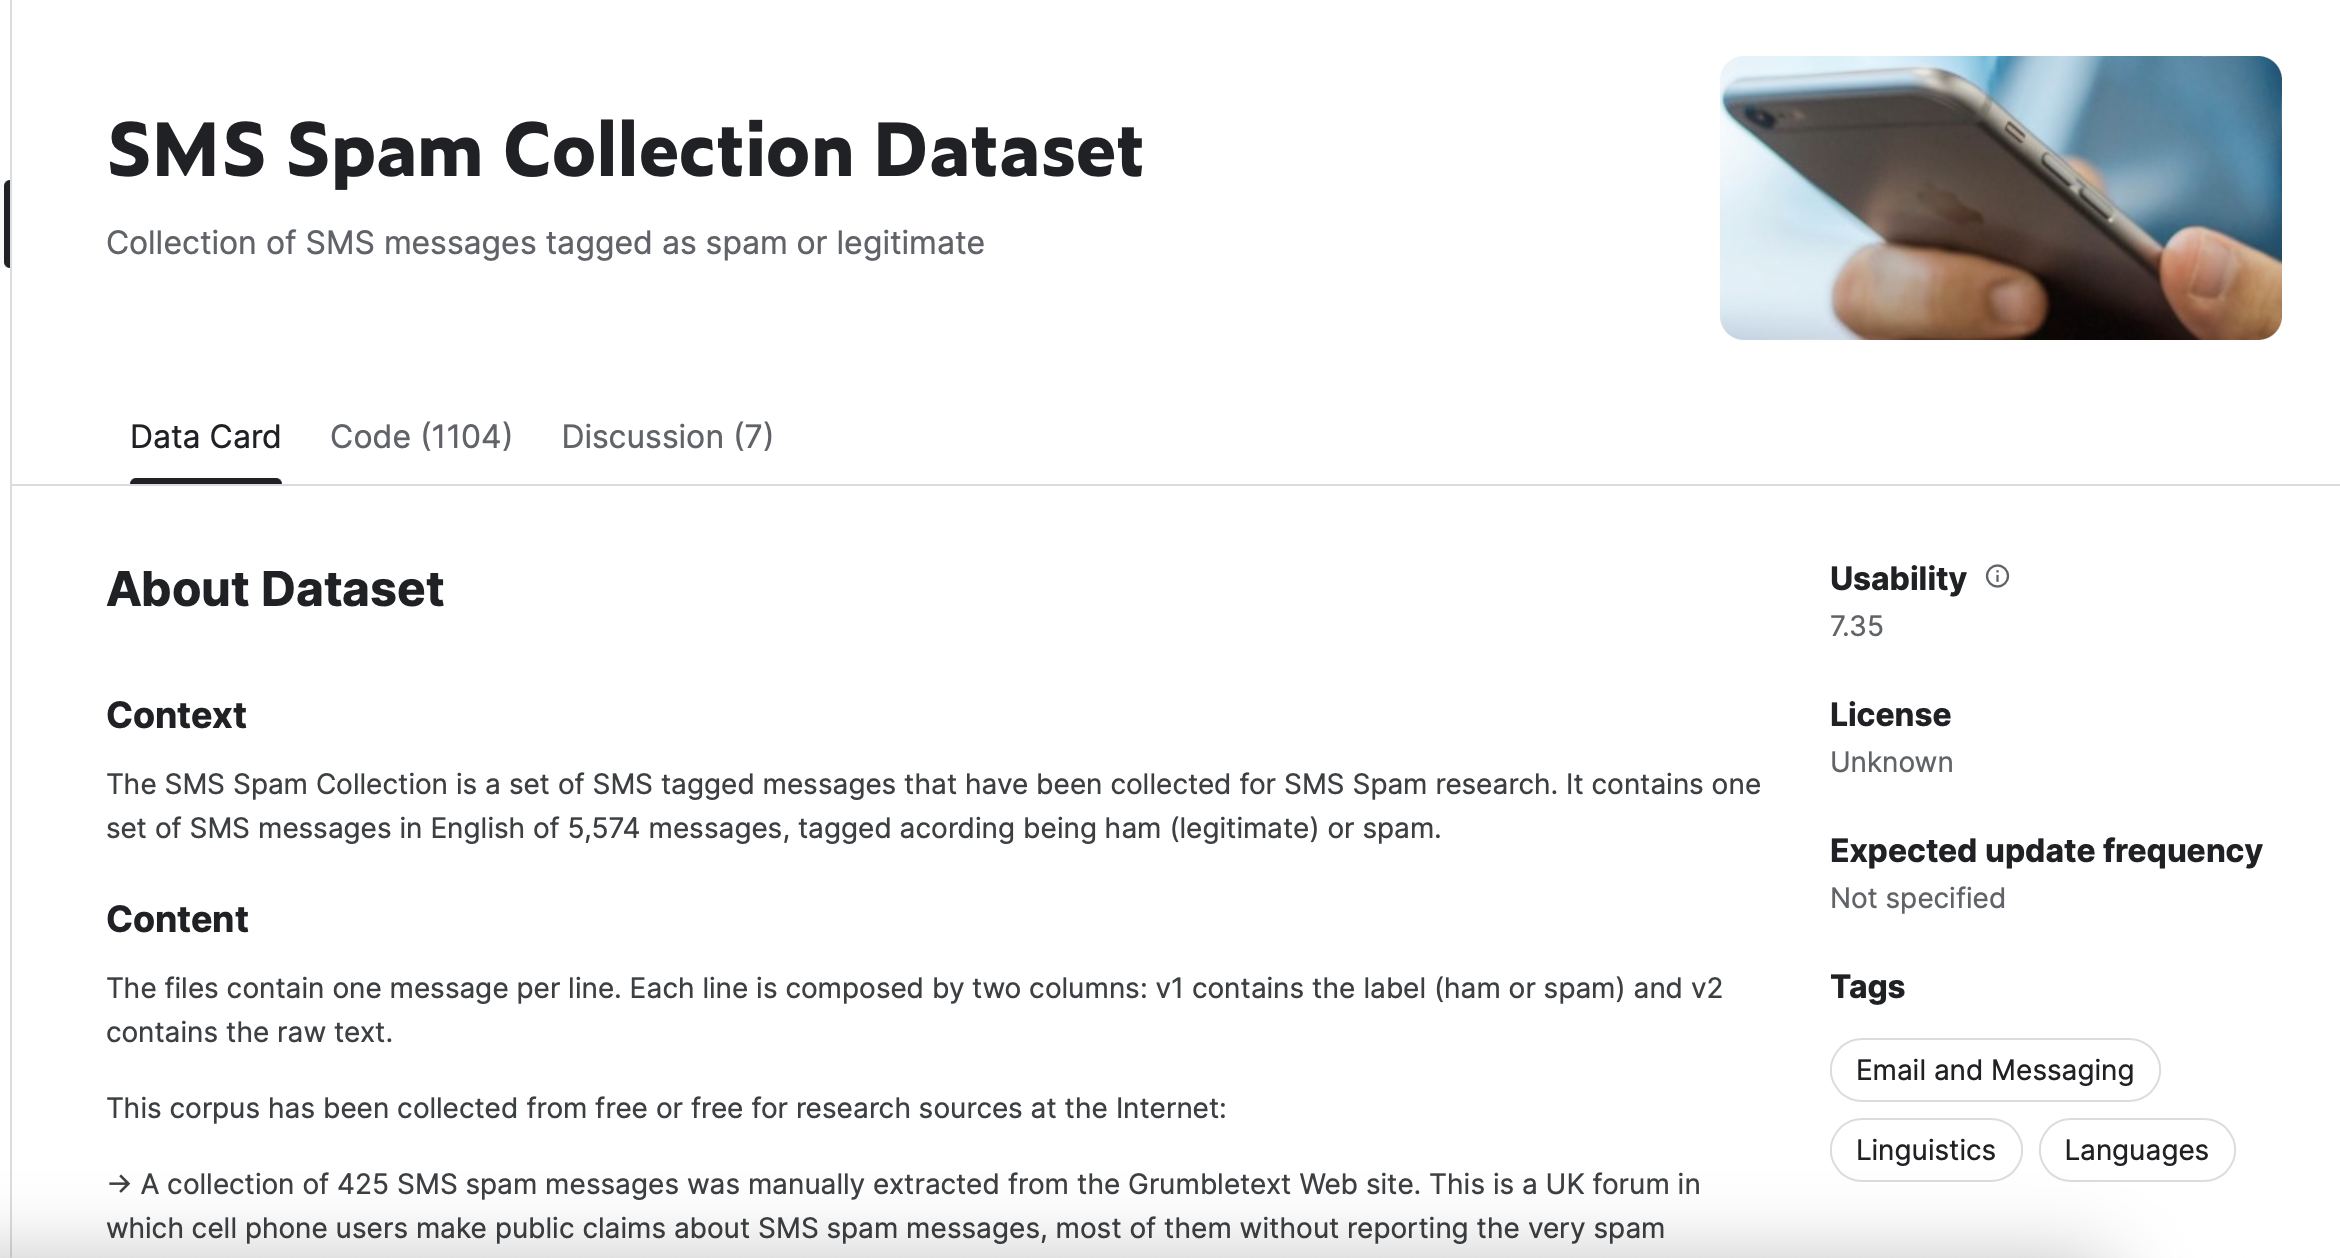
\includegraphics[width=1\linewidth]{images/kaggleDataset.png}
            \caption{Dataset su kaggle.com}
            \label{fig:enter-label}
        \end{figure}

    \subsection{Esplorazione dei dati}
        Il dataset in esame "SMS Spam Collection" è un insieme di messaggi SMS etichettati. Comprende 5.574 messaggi in inglese, suddivisi tra "ham" (legittimi) e "spam". Ogni messaggio è rappresentato da una riga con due colonne: una contiene l'etichetta (ham o spam) ed una contiene il testo grezzo dell'SMS. In questa fase vado ad analizzare, o meglio esplorare più nel dettaglio i dati per comprenderli e per scoprire informazioni rilevanti, tendenze, o relazioni. \\
        Quindi sono andato a fare una prima panoramica del dataset, andando a conteggiare quanti sample per ogni classe (ham/spam) fossero presenti, i nomi delle colonne, per poi passare alla vera esplorazione dei dati, volta quindi a trovare informazioni maggiormente rilevanti.\\
        Per un messaggio di testo è molto interessante andare ad osservare la sua lunghezza, il numero di parole al suo interno ed anche il numero di frasi. Non disponendo di tali feature sono andato a ricavarle, andando ad anticipare la \textbf{feature construction} della fase di Data Preparation.\\
        Per andare a ricavare queste feature dal testo ho utilizzato delle funzioni disponibili nella libreria nltk (conteggio parole e frasi), nonchè la funzione len() per calcolare il numero di caratteri. \\
        Per visualizzare eventuali trend e relazioni tra le varie feature, ho utilizzato alcuni grafici del libreria seaborn. Iniziamo ad analizzare i risultati ottenuti, partendo dal numero di caratteri.

        \begin{figure}[H]
            \centering
            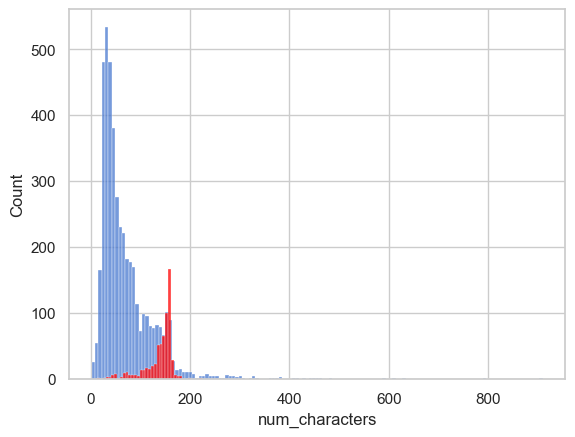
\includegraphics[width=0.6\linewidth]{images/num_char.png}
            \caption{numero di caratteri nei messaggi}
            \label{fig:enter-label}
        \end{figure}

        È da notare che in rosso sono rappresentati gli SMS spam, mentre in blu quelli ham. Sull'asse y la variabile count indica il numero di volte in cui un determinato messaggio ha un certo numero di caratteri. Compreso ciò dal grafico è subito possibile notare che i messaggi spam hanno un numero di caratteri mediamente maggiore dei messaggi ham. \\
        Vediamo ora cosa emerge dal grafico che rappresenta il numero di parole.\\

        \begin{figure}[H]
            \centering
            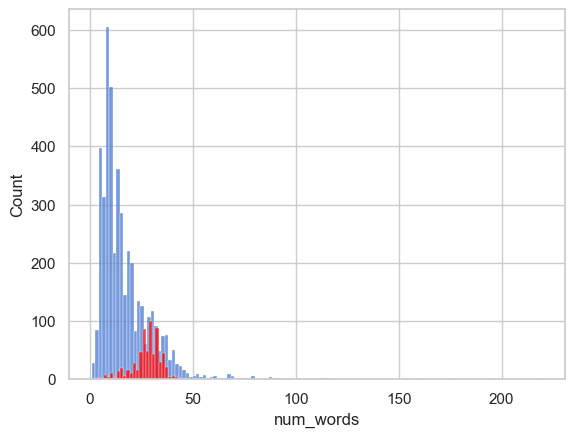
\includegraphics[width=0.6\linewidth]{images/num_words.png}
            \caption{numero di parole nei messaggi}
            \label{fig:enter-label}
        \end{figure}

        Si nota che vale lo stesso per il numero delle parole, difatti per logica il numero di parole è fortemente correlato al numero di caratteri, e quindi sarà facile osservare lo stesso anche per il numero di frasi. Per vedere ancora più chiaramente tale correlazioni sono andato ad utilizzare un grafico riassuntivo, un pairplot, dove ogni variabile numerica presente viene confrontata con tutte le altre variabili numeriche tramite dei grafici a dispersione, che consentono di individuare e visualizzare meglio eventuali relazioni o tendenze.

        \begin{figure}[H]
            \centering
            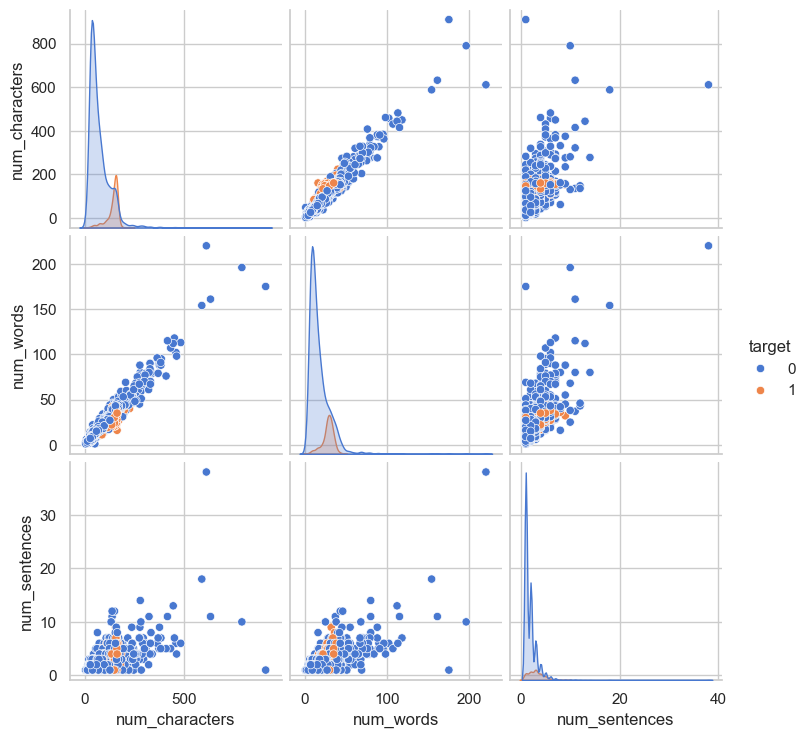
\includegraphics[width=1\linewidth]{images/sns_riassuntivo.png}
            \caption{pairplot riassuntivo}
            \label{fig:enter-label}
        \end{figure}

        Dal grafico emerge, ancora una volta, che:
        \begin{itemize}
        \item gli sms spam hanno in media un numero di caratteri maggiore
        \item gli sms spam hanno in media un numero di parole maggiore
        \end{itemize}

        Per calcolare la correlazione tra le variabili, possiamo usare un'ulteriore strumento: la heatmap, una mappa che utilizza colori per visualizzare i valori dei coefficienti di correlazione tra le diverse coppie di variabili nel dataset, consentendo di individuare facilmente relazioni tra di esse. Le celle più scure o più chiare indicano correlazioni più forti o più deboli, rispettivamente. Le variabili sono fortemente correlate tra loro se hanno valori vicini a 1 o -1, mentre hanno una bassa correlazione se hanno valori vicini a 0.

        \begin{figure}[H]
            \centering
            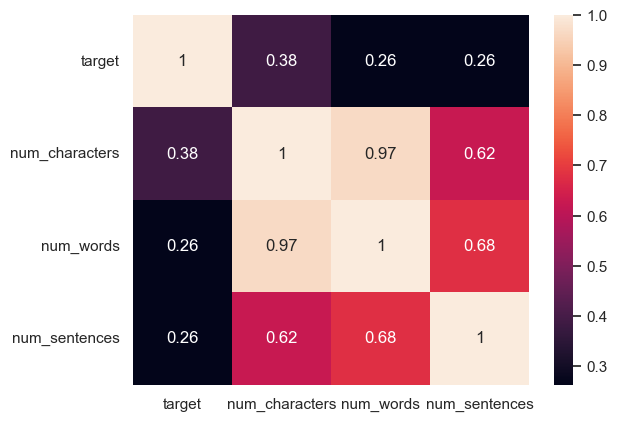
\includegraphics[width=0.7\linewidth]{images/matrice_corr.png}
            \caption{HeatMap}
            \label{fig:enter-label}
        \end{figure}

        E qui possiamo finalmente visualizzare l'effettiva correlazione tra le variabili. Si può notare l'altissima correlazione tra il numero di caratteri e il numero di parole, cosa che è meno marcata con il numero di frasi.\\
        Un'altra cosa davvero molto interessante è andare a visualizzare quali parole sono più frequenti nelle rispettive categoria di messaggi. Per fare ciò ho utilizzato la libreria WordCloud che permette di andare a generare una rappresentazione grafica semplice ed intuitiva. Ecco i due grafici realizzati:

        \begin{figure}[H]
            \centering
            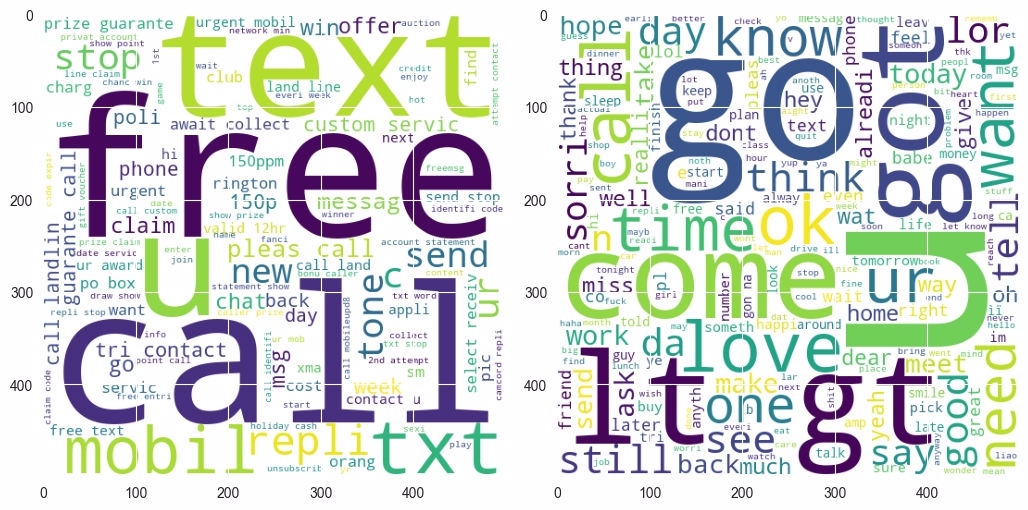
\includegraphics[width=0.7\linewidth]{images/wordCloudSpam.jpg}
            \caption{parole più frequenti (quelle di sinistra si riferiscono ai SPAM, quelle di destra agli HAM)}
            \label{fig:enter-label}
        \end{figure}

        Dai grafici emerge che le parole molto diffuse nei messaggi spam sono "free", "call", "text" e tantissime molte altre parole comuni dei messaggi spam, con lo scopo di fare pubblicità o tanto altro. Nel grafico di destra invece si possono osservare le parole più frequenti nei messaggi ham, e come si può notare sono parole di utilizzo comune, ad esempio c'è anche la parola "ok".

    \subsection{Analisi della qualità dei dati}
        In questa fase vado ad analizzare i problemi di qualità dei dati rilevati durante la fase di esplorazione. A partire dai primi grafici usati nell'esplorazione si può notare che la quantità di messaggi ham, è molto maggiore rispetto alla quantità di messaggi spam.
        Difatti, andando ad approfondire, è risultata la presenza di:
        \begin{itemize}
            \item 4516 sms ham
            \item 653 sms spam
        \end{itemize}
        , graficamente:
        \begin{figure}[H]
            \centering
            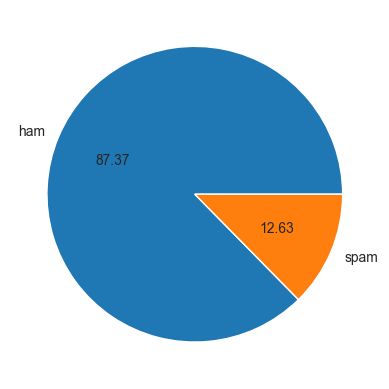
\includegraphics[width=0.5\linewidth]{images/sbilanciamento.png}
            \caption{percentuali di frequenza delle classi}
            \label{fig:enter-label}
        \end{figure}
        Questo indica un forte sbilanciamento dei dati, ed è quindi un problema che dovrà essere risolto. \\
        Altri problemi riscontrati:
        \begin{itemize}
            \item la presenza di 403 messaggi duplicati
            \item due colonne del dataset totalmente nulle
            \item nomi delle colonne non rappresentativi
        \end{itemize}
        Tali problemi saranno risolti nella sezione successiva, ovvero nella \textbf{Data Preparation}.

    \newpage
    \section{Data Preparation}
        Tale fase mira a rendere i dati adatti per l'utilizzo nelle fasi successive del processo. Questo processo include più punti:
        \begin{itemize}
            \item data cleaning
            \item feature scaling
            \item feature selection
            \item data balancing
        \end{itemize}
         Quindi l'output di questa fase sarà un insieme di dati di input, che saranno utilizzati durante la modellazione dell'algoritmo di ML.
    \subsection{Data Cleaning}
        In questa fase vanno corretti i problemi individuati in fase di Data understanding: nel mio caso i valori nulli e duplicati; per poi passare alla trasformazione dei dati in modo da poter essere utilizzati da un algoritmo di apprendimento.\\
        Quindi, innanzitutto, ho eliminato completamente due colonne dal dataset poiché erano completamente vuote, ed ho rinominato le colonne "target" e "text" in quanto i nomi precedenti ("v1", "v2") erano ambigui e poco rappresentativi. Successivamente, ho rimosso 403 valori duplicati e ho sostituito le stringhe "spam" e "ham" della variabile target rispettivamente con i valori 1 e 0, per garantire la compatibilità con gli algoritmi di classificazione binaria.

        Avendo a che fare con del testo, ho effettuato la fase di "mining", ovvero l'estrazione di semantica dai testi, che va adattata al contesto. I maggiori problemi da affrontare riguardano il fatto che nel linguaggio naturale son presenti più modi per esprimere stessi concetti, possono esserci errori grammaticali; o più in generale l'estrazione delle informazioni viene difficile. Nel mio caso trattandosi di testo di messaggi, ho deciso di attuare le seguenti trasformazioni:
        \begin{itemize}
            \item Tokenizzazione
            \item Portato tutto in minuscolo
            \item Rimosso i caratteri non alfanumerici
            \item Rimosso le stopwords
            \item Stemming
        \end{itemize}
        Tutte queste trasformazioni effettuate hanno scopi ben precisi; infatti la \textbf{tokenizzazione} aiuta a trattare le parole individualmente durante l'analisi;
        \textbf{portare tutto in minuscolo} aiuta ad eliminare la distinzione tra maiuscole e minuscole, garantendo coerenza nell'analisi; la \textbf{rimozione caratteri non alfanumerici} va ad eliminare simboli e punteggiatura concentrando l'attenzione sulle informazioni sostanziali delle parole; la \textbf{rimozione delle stopwords} che sono parole comuni che non contribuiscono significativamente al significato aiuta a ridurre il rumore nei dati; ed infine lo \textbf{stemming} che riduce le parole alle loro radici (stems) fa in modo che parole simili siano rappresentate in modo uniforme, semplificando l'analisi.
        Ho realizzato ciò usando funzioni e dizionari preesistenti, andando solamente ad accorpare il tutto in un'unica funzione.
        \newpage
        \begin{verbatim}

            def transform_text(text):
                text = text.lower() #tutto in minuscolo
                text = nltk.word_tokenize(text) #tokenizzazione

                #Rimozione caratteri non alfanumerici
                y = []
                for i in text:
                    if i.isalnum():
                        y.append(i)

                text = y[:]
                y.clear()

                # Rimozione stopwords
                for i in text:
                    if i not in stopwords.words('english') and i not in string.punctuation:
                        y.append(i)

                text = y[:]
                y.clear()

                #stemming (ps è l'oggetto portStemmer)
                for i in text:
                    y.append(ps.stem(i))

                #Restituisce il testo pre-elaborato come una stringa di parole separate tra spazi.
                return " ".join(y)

        \end{verbatim}
        Quindi dopo aver definito tale funzione, ho semplicemente processato tutto il testo degli SMS per poi inserirlo in una nuova colonna del dataset.

    \subsection{Feature Scaling}
        In questa fase si vanno ad utilizzare delle tecniche per normalizzare o scalare i valori delle caratteristiche in modo da avere una scala uniforme. Questo serve per evitare che caratteristiche con scale molto diverse influenzino negativamente gli algoritmi di apprendimento. Nel mio caso ho notato che le scale fra il numero di caratteri, numero di parole e numero di frasi sono molto differenti; difatti i caratteri arrivano anche a oltre 180, il numero di parole non supera nella maggiorparte dei casi 50, ed infine il numero frasi non supera le 10. Quindi ho ritenuto opportuno andare a normalizzare tali valori, e per farlo ho usato una funzione della libreria sklearn.
        \begin{verbatim}
            #colonne che voglio normalizzare
            features_to_normalize = ['num_characters', 'num_words', 'num_sentences']

            #oggetto che permette la normalizzazione
            scaler = MinMaxScaler()

            df[features_to_normalize] = scaler.fit_transform(df[features_to_normalize])
        \end{verbatim}

        \subsection{Feature Selection}
            La feature selection è il processo in cui si va a scegliere un sottoinsieme delle caratteristiche più rilevanti dai dati originali per andare a ridurre la complessità del modello. Qui entra in gioco il \textbf{Feature Engineering} ovvero il processo nel quale il progettista utilizza la propria conoscenza del dominio per determinare le feature e dare più o meno enfasi ad esse. Nel mio caso, osservando i valori dopo, o comunque prima della fase di Feature Scaling, ho notato che: il numero di frasi dei messaggi è una feature a bassa varianza (ovvero i suoi valori variano poco) quindi tale feature è non rilevante per la classificazione; di conseguenza ho deciso di eliminarla. In questa fase si vanno anche ad effettuare altre operazioni, come ad esempio la \textbf{feature construction}, in cui il progettista va a costruire nuove caratteristiche a partire dai dati. Personalmente ho costruito in precedenza due feature, difatti partendo dal testo ho ricavato il numero di frasi, di parole e di caratteri.

        \subsection{Data Balancing}
            Il Data Balancing si riferisce alle tecniche usate per convertire un dataset sbilanciato in un uno bilanciato. Avere un dataset sbilanciato può portare a diversi problemi, tra questi previsioni sbilanciate e innaccurate, nonchè problematiche di overfitting.
            Le tecniche applicabili sono due:
            \begin{itemize}
                \item Undersampling
                \item Oversampling
            \end{itemize}
            con la presenza di varianti che includono il clustering, per evitare alcuni inconvenienti, come ad esempio andare ad eliminare righe molto utili per l'apprendimento. Nel mio caso, il dataset è fortemente sbilanciato, con una presenza maggiore di istanze della classe ham. Quindi le possibilità sono due:
            \begin{itemize}
                \item Eliminare istanze della classe ham
                \item Aumentare le istanze della classe spam
            \end{itemize}
            Tra le due, per evitare troppa duplicazione e quindi probabile overfitting, ho deciso di optare per la prima opzione, andando a considerare l'uso dell' \textbf{undersampling con clustering}, per evitare appunto di eliminare istanze particolarmente rilevanti per l'apprendimento.\\
            Per quanto riguarda l'algoritmo di clustering da utilizzare ho optato per il k-means, l'algoritmo a partizionamento iterativo più diffuso, per principalmente due motivi: la forma della distribuzione dei dati, e la presenza di pochi outlier, che in parte ho deciso di eliminare. Per individuare ed eliminare gli outlier ho calcolato media e deviazione standard, per poi eliminare tutte le istanze che distano 4 deviazioni standard dalle media.\\
            Per la configurazione del k-means c'è un parametro di vitale importanza: k, ovvero il numero di cluster da generare. Non sapendo che valore assegnare a tale parametro ho optato nella valutazione di due tecniche:
            \begin{itemize}
                \item Elbow Point
                \item Silhouette score
            \end{itemize}

            \subsubsection{Elbow Point}
                Il punto di gomito è un metodo empirico, che consiste nel graficare i valori candidati del parametro k rispetto alla somma degli errori quadratici ottenuti dall’algoritmo configurato per generare k cluster.
                \begin{figure}[H]
                    \centering
                    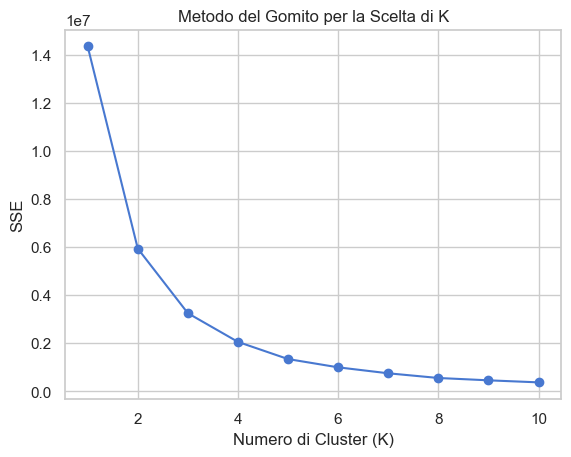
\includegraphics[width=0.7\linewidth]{images/elbowPoint.png}
                    \label{fig:enter-label}
                \end{figure}
                Come si può notare dal grafico, il numero ideale di cluster suggerito è tra 4 e 5. Ho successivamente provato anche il silhoette coefficient per avere un'ulteriore confronto.

            \subsubsection{Silhouette Coefficient}
                È una misura della coesione e separazione tra i dati. Più in particolare, quantifica quanto i dati siano ben disposti nei cluster generati; in particolare si basa su quanto bene i dati sono ammassati nel cluster e quanto è distante ciascun campione da qualsiasi altro cluster. Tale coefficiente varia tra -1 e +1 e i valori alti indicano maggiore coesione e separazione dei dati.
                \begin{figure}[H]
                    \centering
                    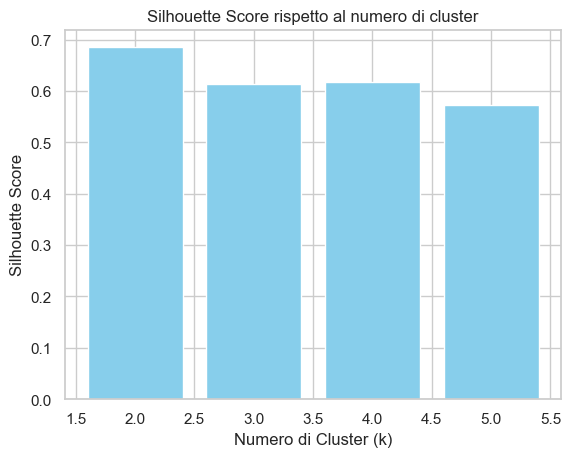
\includegraphics[width=0.6\linewidth]{images/silhouetteScores.png}
                    \label{fig:enter-label}
                \end{figure}
                Anche qui ho usato una valutazione empirica, ovvero ho eseguito il k-means con diversi valori di k (2, 3, 4, 5) e ho osservato che il silhouette coefficient è maggiore per k = 2.

            \subsubsection{Scelta del k}
                Quindi ho ottenuto valori discordanti dalle due metodologie usate:
                \begin{itemize}
                    \item Elbow Point: k=3 o k=4
                    \item Silhouette score: k=2
                \end{itemize}
                Quindi per andare a decidere il valore da assegnare a k, ho eseguito tutti i passi successivi (modeling, evaluation) per k=2, 3, 4. Ho osservato  risultati migliori per k=2.\\

            \subsubsection{Clustering con k=2}
                Una volta individuato il miglior valore per k sono andato ad eseguire in maniera definitiva il clustering.
                \begin{figure}[H]
                    \centering
                    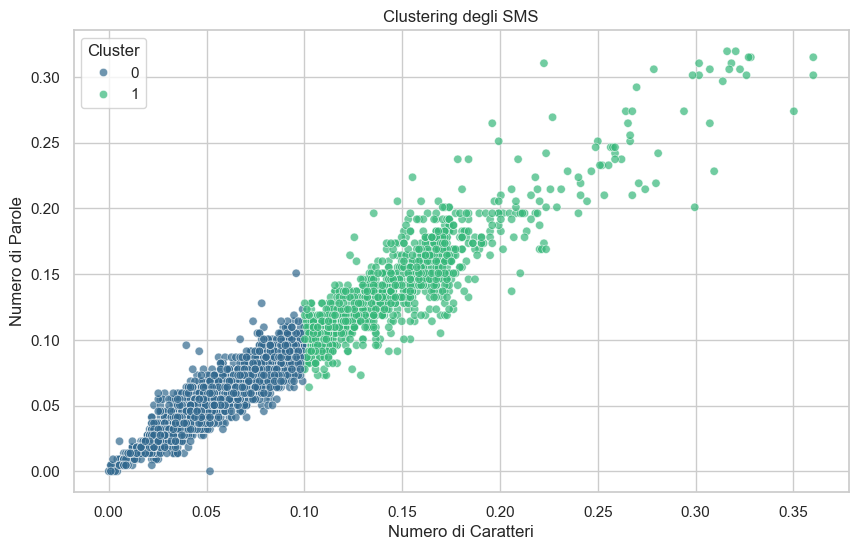
\includegraphics[width=0.9\linewidth]{images/clust.png}
                    \caption{k-means con k=2, dopo la rimozione degli outlier}
                    \label{fig:enter-label}
                \end{figure}

            \subsubsection{Selezione campioni dai cluster}
                Una volta effettuato il clustering, e aver creato due cluster distinti ho selezionato casualmente 325 istanze per ogni cluster, in modo da avere un totale di 650 sms ham. In questo modo ho quasi lo stesso numero di messaggi per ogni classe.

                \begin{figure}[H]
                    \centering
                    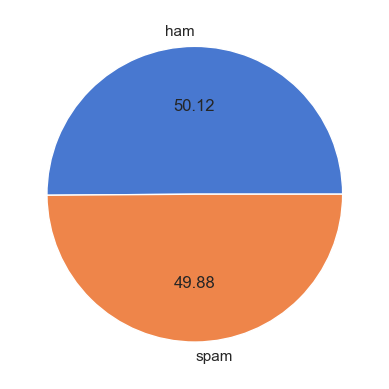
\includegraphics[width=0.5\linewidth]{images/datasetBilanciato.png}
                    \caption{Frequenza delle classi dopo la fase di Undersampling}
                    \label{fig:enter-label}
                \end{figure}



        \subsection{Rappresentazione Numerica dei Dati Testuali}
            Prima di procedere con la fase di modeling, sono necessarie alcuni passaggi finali, tra questi: trasformazione dei dati in rappresentazione numerica e split del dataset. La ragione della prima operazione risiede nel fatto che la maggior parte degli algoritmi di apprendimento richiede in input dati in formato numerico.\\
            Usando il TfidfVectorizer ho trasformato i dati testuali in una rappresentazione numerica, successivamente ho combinato l'output di tale operazione con le feature già numeriche (numero parole, numero caratteri), per poi procedere, allo split del dataset.

        \subsection{Split del Dataset}
            Come ribadito precedentemente, prima di passare alla fase di modeling c'è bisogno di andare ad effettuare lo split del dataset, ovvero dividere il l'insieme di partenza in due sottoinsiemi: uno per l'addestramento ed uno per il testing. Difatti andare ad addestrare e testare un modello sugli stessi dati porta ad avere risultati inaffidabili.\\
            Per fare tale operazione mi sono affidato alla libreria sickitLearn, ed in particolare al 'train test split'.
            Dopo questo i dati sono finalmente pronti per essere dati in input ad un modello di Machine Learning.

        \newpage
        \section{Data Modeling}
            Nella sezione precedente ho preparato i dati in modo da essere dati in input ad un algortimo, quindi può iniziare la fase di modeling. Per prima cosa va quindi selezionato l’algoritmo da
            utilizzare per poi passare alla fase di addestramento, dove si addestra il modello e di conseguenza si descrivono i risultati ottenuti.

            \subsection{Scelta dell'algoritmo}
                SMSecure va quindi a trattare un problema di apprendimento supervisionato, e più nel dettaglio un problema di classificazione. Difatti verrà fornito all'algoritmo un insieme di dati con rispettivo valore della variabile target, ed inoltre la variabile target potrà assumere solamente un numero discreto di valori, nello specifico solamente due: 0 per "ham" e 1 per "spam". Quindi i possibili algoritmi utilizzabili sono i seguenti: Regressione Logistica, Support Vector Machines, K-Nearest Neighbors, Random Forest, Naive Bayes e gli Alberi Decisionali (DTC).\\
                Tuttavia ho concentrato la mia scelta solo sui due algortimi visti a lezione, ovvero:
                \begin{itemize}
                    \item Naive Bayes
                    \item Alberi Decisionali (DTC)
                \end{itemize}
                Questi sono due algoritmi che operano in maniera differente per arrivare alla classificazione: infatti il primo considera le caratteristiche della nuova istanza da classificare e calcola la probabilità che queste facciano parte di una classe tramite l’applicazione del teorema di Bayes, mentre il secondo mira a creare un albero i cui nodi rappresentano un sotto-insieme di caratteristiche del problema e i cui archi rappresentano delle decisioni; il tutto sfruttando i concetti di Entropia e Information-Gain utili per andare a suddividere l'insieme di partenza.\\
                In linea generale, gli Alberi Decisionali sono noti per la loro flessibilità nel catturare relazioni complesse nei dati, mentre il classificatore Naive Bayes eccelle per la sua velocità di addestramento, efficacia nei dati testuali. Poiché non sono un esperto di algoritmi e non posso prevedere quale si adatti meglio al mio problema, ho adottato la valutazione empirica:  ovvero l'addestramento del modello prima con un Naive Bayes e successivamente con Decision Tree, per poi valutare e confrontare i risultati ottenuti. In questo modo riesco a determinare quale algoritmo si comporta meglio rispetto ai miei obiettivi e procedere quindi all'export.

            \subsection{Addestramento}
                In questa sezione procedo ad addestrare il modello in base all'algoritmo scelto in precedenza. Nel mio caso, come già detto,  procedo prima all'addestramento usando Naive Bayes, per poi fare lo stesso con Decision Tree. Infine valuterò le prestazioni ottenute e le metterò a confronto. Tutto ciò mi consentirà di capire quale algoritmo si adatta meglio ai dati, e va di conseguenza a fare delle predizioni migliori.\\

                \subsubsection{Naive Bayes}
                    L'algoritmo Naive Bayes \cite{wikiNaiveBayes} è un algoritmo di classificazione basato sul teorema di Bayes, che riguarda la probabilità condizionata. Si parla di  "naive" perchè tale algortimo considera l'indipendenza tra le caratteristiche, ciò semplifica i calcoli e rende l'algoritmo veloce. Ci sono diverse varianti del Naive Bayes, tra cui:
                    \begin{itemize}
                        \item Multinomial Naive Bayes (MNB)
                        \item  Gaussian Naive Bayes (GNB)
                        \item Bernoulli Naive Bayes (BNB)
                    \end{itemize}
                    Tali differiscono nelle loro ipotesi sulla distribuzione delle caratteristiche, ovvero la probabilità delle diverse features condizionate alle classi di output. Ad esempio l'MNB è particolarmente utile per problemi di classificazione di testi, il GNB per dati continui, ed infine il BNB per dati binari. Anche qui ho adottato la valutazione empirica, andandoli a provare tutti! \\
                    Queste sono le matrici di confusione che ho ottenuto:
                    \begin{figure}[H]
                        \centering
                        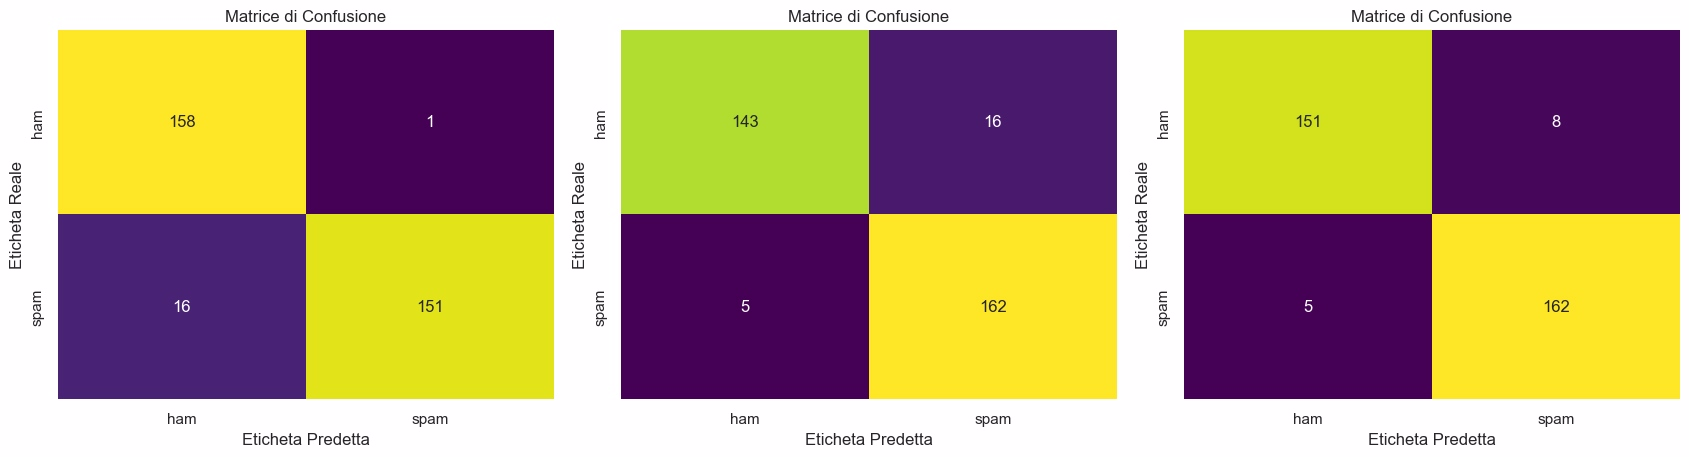
\includegraphics[width=1\linewidth]{images/naiveBayesResults.jpg}
                        \caption{Risultati BNB, GNB, MNB. Rispettivamente in questo ordine}
                        \label{fig:enter-label}
                    \end{figure}
                    Successivamente a partire dalle matrici di confusione, che esprimono al loro interno il numero di True Positive (alto a sinistra), True Negative (basso a destra), False Positive (alto a destra), False Negative (basso a sinistra) sono andato anche a calcolare alcune metriche di valutazione, ovvero Precisione, Recall e Accuratezza; che vanno calcolate proprio usando gli indicatori espressi dalle matrici. Il mio obiettivo è andare a massimizzare tutte e tre le metriche.\\
                    Risultati ottenuti:
                    \begin{figure}[H]
                        \centering
                        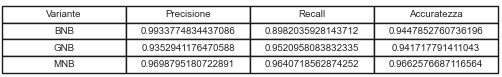
\includegraphics[width=1\linewidth]{images/resultTableNaiveBayes.png}
                        \label{fig:enter-label}
                    \end{figure}
                    Andiamo a fare un'analisi dei risultati ottenuti, ma prima vediamo cosa esprimono nel mio caso tali indicatori.
                    \begin{itemize}
                        \item La \textbf{Recall} rappresenta la proporzione di messaggi spam che sono stati correttamente identificati rispetto al totale dei messaggi spam effettivi. Un valore elevato indica che il modello è in grado di individuare la maggior parte dei messaggi spam.
                        \item La \textbf{Precisione} rappresenta la proporzione di messaggi classificati come spam che sono effettivamente spam. Un valore elevato indica che il modello ha pochi falsi positivi, cioè pochi messaggi ham erroneamente classificati come spam.
                        \item L'\textbf{accuratezza} rappresenta la proporzione di tutte le previsioni corrette (veri positivi e veri negativi) rispetto a tutte le previsioni fatte dal modello. Tale indicatore, come visto a lezione, può essere influenzato dallo sbilanciamento dei dati; non è questo il caso dato che ho provveduto precedentemente a bilanciare i dati.
                    \end{itemize}
                    Da come emerge dai valori ottenuti, il classificatore Naive Bayes MNB ha ottenuto ottimi risultati su tutte le metriche. Una particolarità osservabile è che il Naive Bayes BNB ha ottenuto una precisione molto alta, a sfavore di una recall piuttosto bassa rispetto gli altri. Dal mio punto di vista è meglio avere una recall il più alta possibile, difatti preferirei che qualche messaggio ham venga erroneamente classificato rispetto al ricevere fastidiosi sms spam. Quindi tra i tre preliligo il classificatore MNB.
                    Andiamo ora ad addestrare il modello usando il Decision Tree.

                \subsubsection{Decision Tree}
                    Il DTC \cite{wikiDTC} è un classificatore che opera attraverso una struttura ad albero. Ogni nodo rappresenta un sottoinsieme delle caratteristiche, e i rami che si dipartono da ogni nodo indicano i possibili valori di quelle caratteristiche.
                    Il processo di costruzione dell'albero inizia con la scelta della caratteristica che meglio divide il set di dati in classi omogenee, ciò viene fatto utilizzando misure come l'entropia o l'information-gain (misura quanto un attributo divide bene il dataset). Una volta individuata la caratteristica deve essere creato un nodo e  diviso il set di dati in base ai possibili valori di quella caratteristica. Ciò viene quindi ripetuto su ciascun sottoinsieme di dati, creando ulteriori nodi e rami
                    fin quando viene raggiunto un criterio di stop o si arriva ad avere dei set puri, ovvero composti esclusivamente da istanze di un'unica classe.
                    Dopo l'addestramento ho testato il modello, e questa è la matrice di confusione ottenuta:
                    \begin{figure}[H]
                        \centering
                        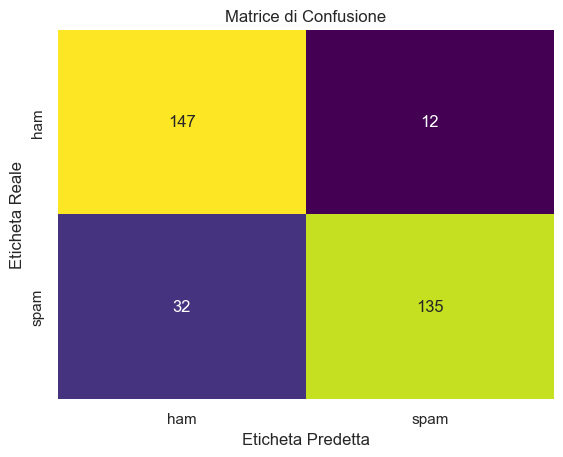
\includegraphics[width=0.6\linewidth]{images/dtcResult.png}
                        \caption{Matrice confusione DTC (maxDepth=8)}
                        \label{fig:enter-label}
                    \end{figure}
                    È da notare che l'algoritmo DTC ha un importante parametro: maxDepth, ovvero il numero massimo di livelli creati per l'albero. Per trovare la profondità massima ottimale ho rieseguito l'algoritmo più volte, andando a variare il parametro. Ho osservato che le performance in termini di precisione/accuratezza/recall sono aumentate fino ad una profondità pari ad 8, per poi andare in stallo o peggiorare.

                    \subsubsection{MNB vs DTC}

                        \begin{figure}[H]
                            \centering
                            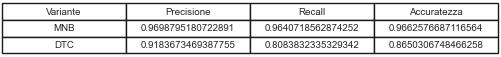
\includegraphics[width=1\linewidth]{images/FinalTable.png}
                            \label{fig:enter-label}
                        \end{figure}

                        Come si può notare i risultati ottenuti  usando il DTC non sono dei migliori. Ciò probabilmente è dovuto a più fattori, in particolare  alla grandezza del dataset, difatti dopo il bilanciamento ho solamente 650 entry per classe. Quindi la discrepanza tra le due valutazioni potrebbe essere data dal differente modo di operare dei due algoritmi. Per sua natura il Naive Bayes semplifica la complessità del problema assumendo un'indipendenza tra le varie caratteristiche, quindi nel contesto dei messaggi considererà la probabilità di trovare una certa parola in un messaggio, di conseguenza se una parola specifica è spesso associata ai messaggi spam in addestramento, allora il modello imparerà tale relazione e utilizzerà queste informazioni per fare predizioni su nuove istanze. Conseguenza di quanto detto è che il Naive Bayes si adatta facilmente a situazioni in cui ci sono relativamente pochi dati, cosa che non fa il Decision Tree.
                        Questo è un grafico che riporta i risultati ottenuti da tutti gli addestramenti svolti:
                        \begin{figure}[H]
                            \centering
                            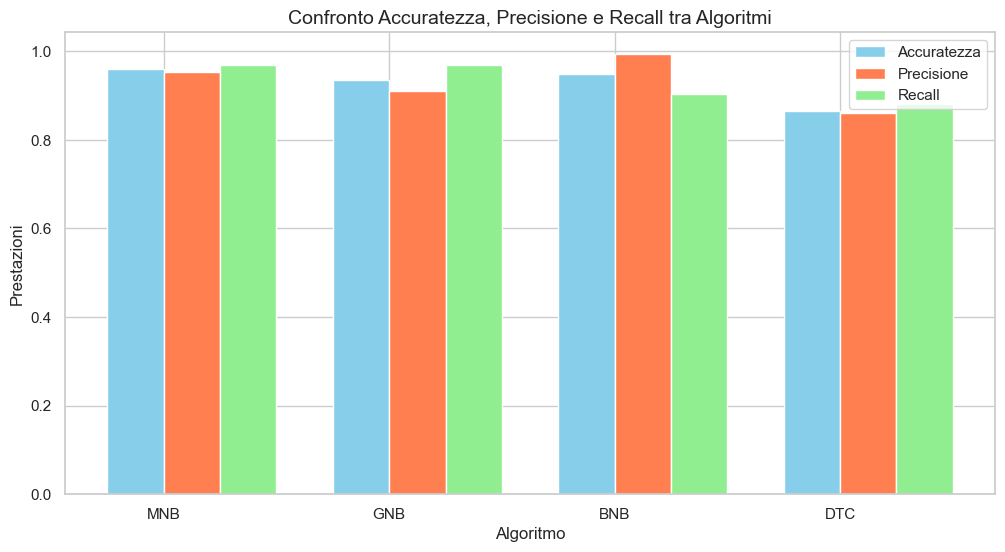
\includegraphics[width=1\linewidth]{images/AllResult.png}
                            \label{fig:enter-label}
                        \end{figure}
                        Come emerge l'algoritmo che si è comportato meglio è stato il Naive Bayes MNB.
        \newpage
        \section{Evaluation}
            In questa fase si va a valutare se i
            risultati sono chiari, se sono in linea con gli obiettivi e se rivelano delle prospettive aggiuntive
            alle quali non si era pensato, nonchè verificare la consistenza e la solidità dell’intero processo.
            Vado quindi ad esaminare più nel dettaglio i risultati che ho ottenuto
            dall'addestramento e dal testing  del Naive Bayes MNB, che ha avuto le seguenti performance:
            \begin{figure}[H]
                \centering
                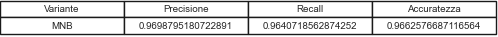
\includegraphics[width=1\linewidth]{images/MNBresult.png}
                \label{fig:enter-label}
            \end{figure}
             Per avere più chiara la bontà del modello ho effettuato un'ulteriore valutazione attraverso la ROC-AUC curve, che consente di visualizzare il trade-off tra Recall e specificità. In poche parole misura la capacità di identificare correttamente i casi negativi, ovvero quanto bene il modello riesce a distinguere tra messaggi ham e spam.
             \begin{figure}[H]
                 \centering
                 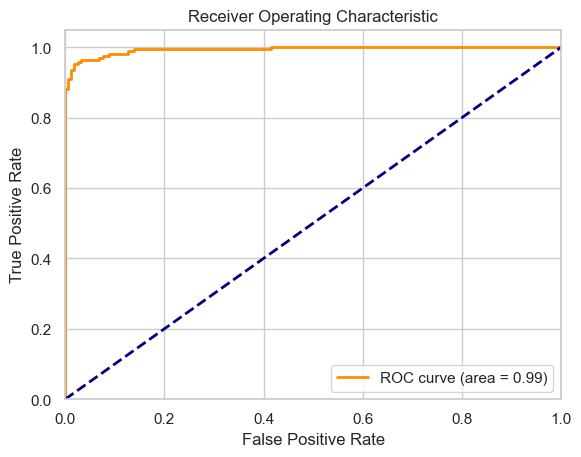
\includegraphics[width=0.6\linewidth]{images/ROC-AUC.png}
                 \label{fig:enter-label}
             \end{figure}
             La linea diagonale rappresenta il risultato di una scelta casuale, quindi un qualunque modello utile deve essere al suo di sopra. Nel mio caso è proprio così. Inoltre un buon modello deve posizionarsi in alto a sinistra, ovvero deve avere sensibilità elevata e basso tasso di falsi positivi, cioè il modello deve riuscire a classificare correttamente la maggior parte dei messagi spam senza generare falsi positivi, ovvero ham classificati come spam. Ultima non meno importante la AUC (Area sotto la curva) che fornisce una misura generale delle prestazioni del modello, ad esempio un'area di 1.0 indica un modello perfetto, mentre un'area di 0.5 indica una scelta casuale. Il mio modello ha ottenuto un valore pari a 0.99, che è un ottimo risultato.
             Quindi posso considerare la costruzione del modello e in generale dell'approccio completa.

        \newpage
        \section{Deployment}
            La fase di deployment rappresenta il culmine dell'intero processo di sviluppo di un modello di ML, si va quindi a trasformare il modello addestrato in una soluzione pronta per l'uso. Quindi ho dovuto esportare il modello precedentemente addestrato, per integrarlo in una semplice applicazione. L'idea per questa applicazione è la seguente: una semplice text area in cui l'utente può inserire il testo del messaggio ricevuto, e premendo un apposito pulsante, verrà visualizzata la predizione del sistema. Inoltre verrà anche mantenuta la history dei messaggi, fino alla chiusura della schermata. Per realizzare ciò ho utilizzato la libreria Streamlit, adatta alla creazione di veloci web app.
            \begin{figure}[H]
                \centering
                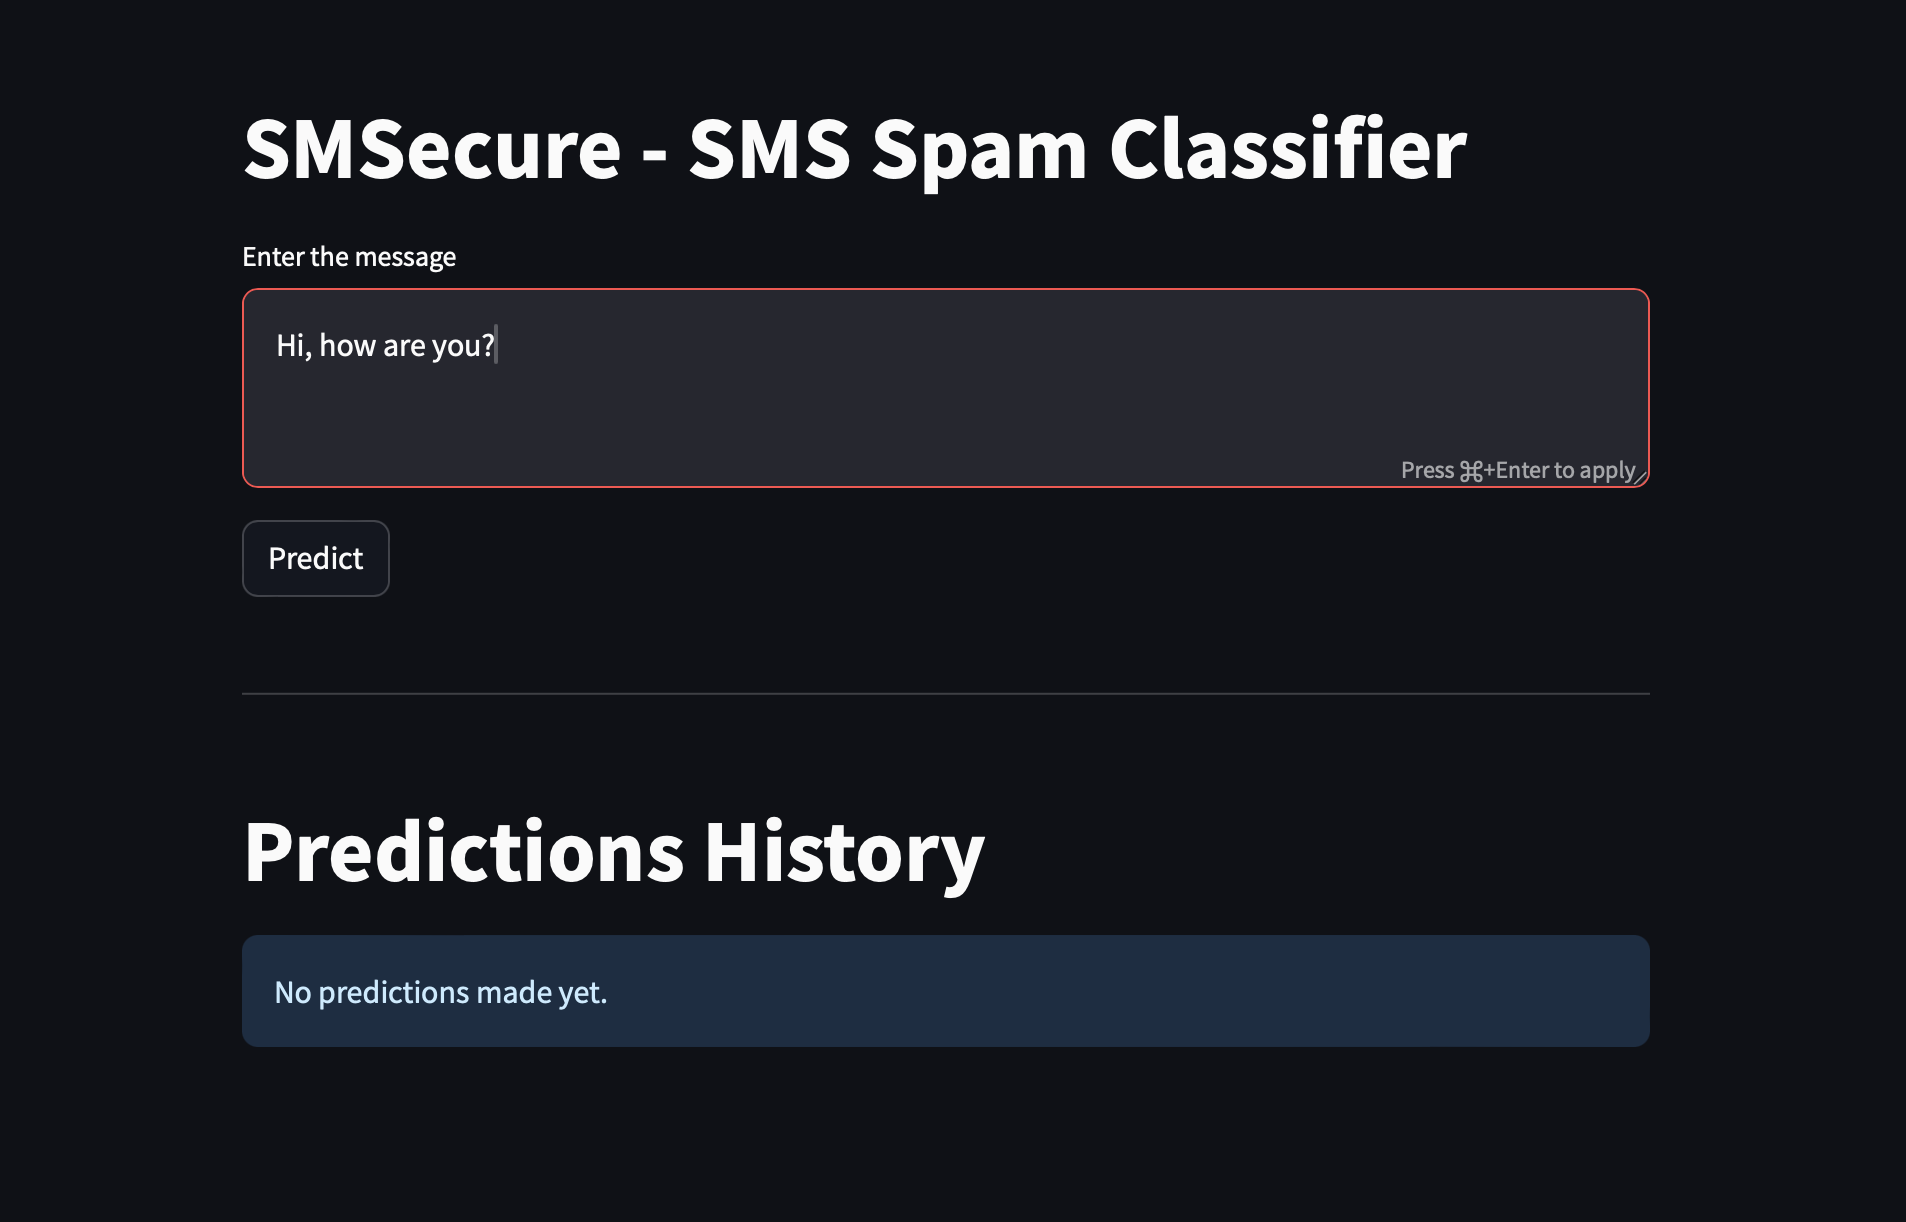
\includegraphics[width=1\linewidth]{images/app.png}
                \caption{SMSecure app [schermata di apertura]}
                \label{fig:enter-label}
            \end{figure}
            L'app inoltre, una volta che viene fatta una predizione va anche a visualizzare eventuali parole individuate che frequentemente appaiono in messaggi ham o spam.
            Per realizzare ciò, ho quindi dovuto esportare oltre al modello addestrato, anche il tfidf, in modo da garantire che la rappresentazione dei dati utilizzata durante l'addestramento sia coerente con quella utilizzata durante il deployment, ed anche la frequenza di parole ham/spam. Per garantire coerenza nell'intero processo non è bastato solamente andare ad usare lo stesso vectorizer, ma ho dovuto eseguire sul messaggio inserito dall'utente tutte le operazioni che ho fatto in fase di addestramento, dalla data preparation alla trasformazione del testo in dati numerici, andando anche a ricavare dal testo il numero di parole e il numero di caratteri.
            \begin{figure}[H]
                \centering
                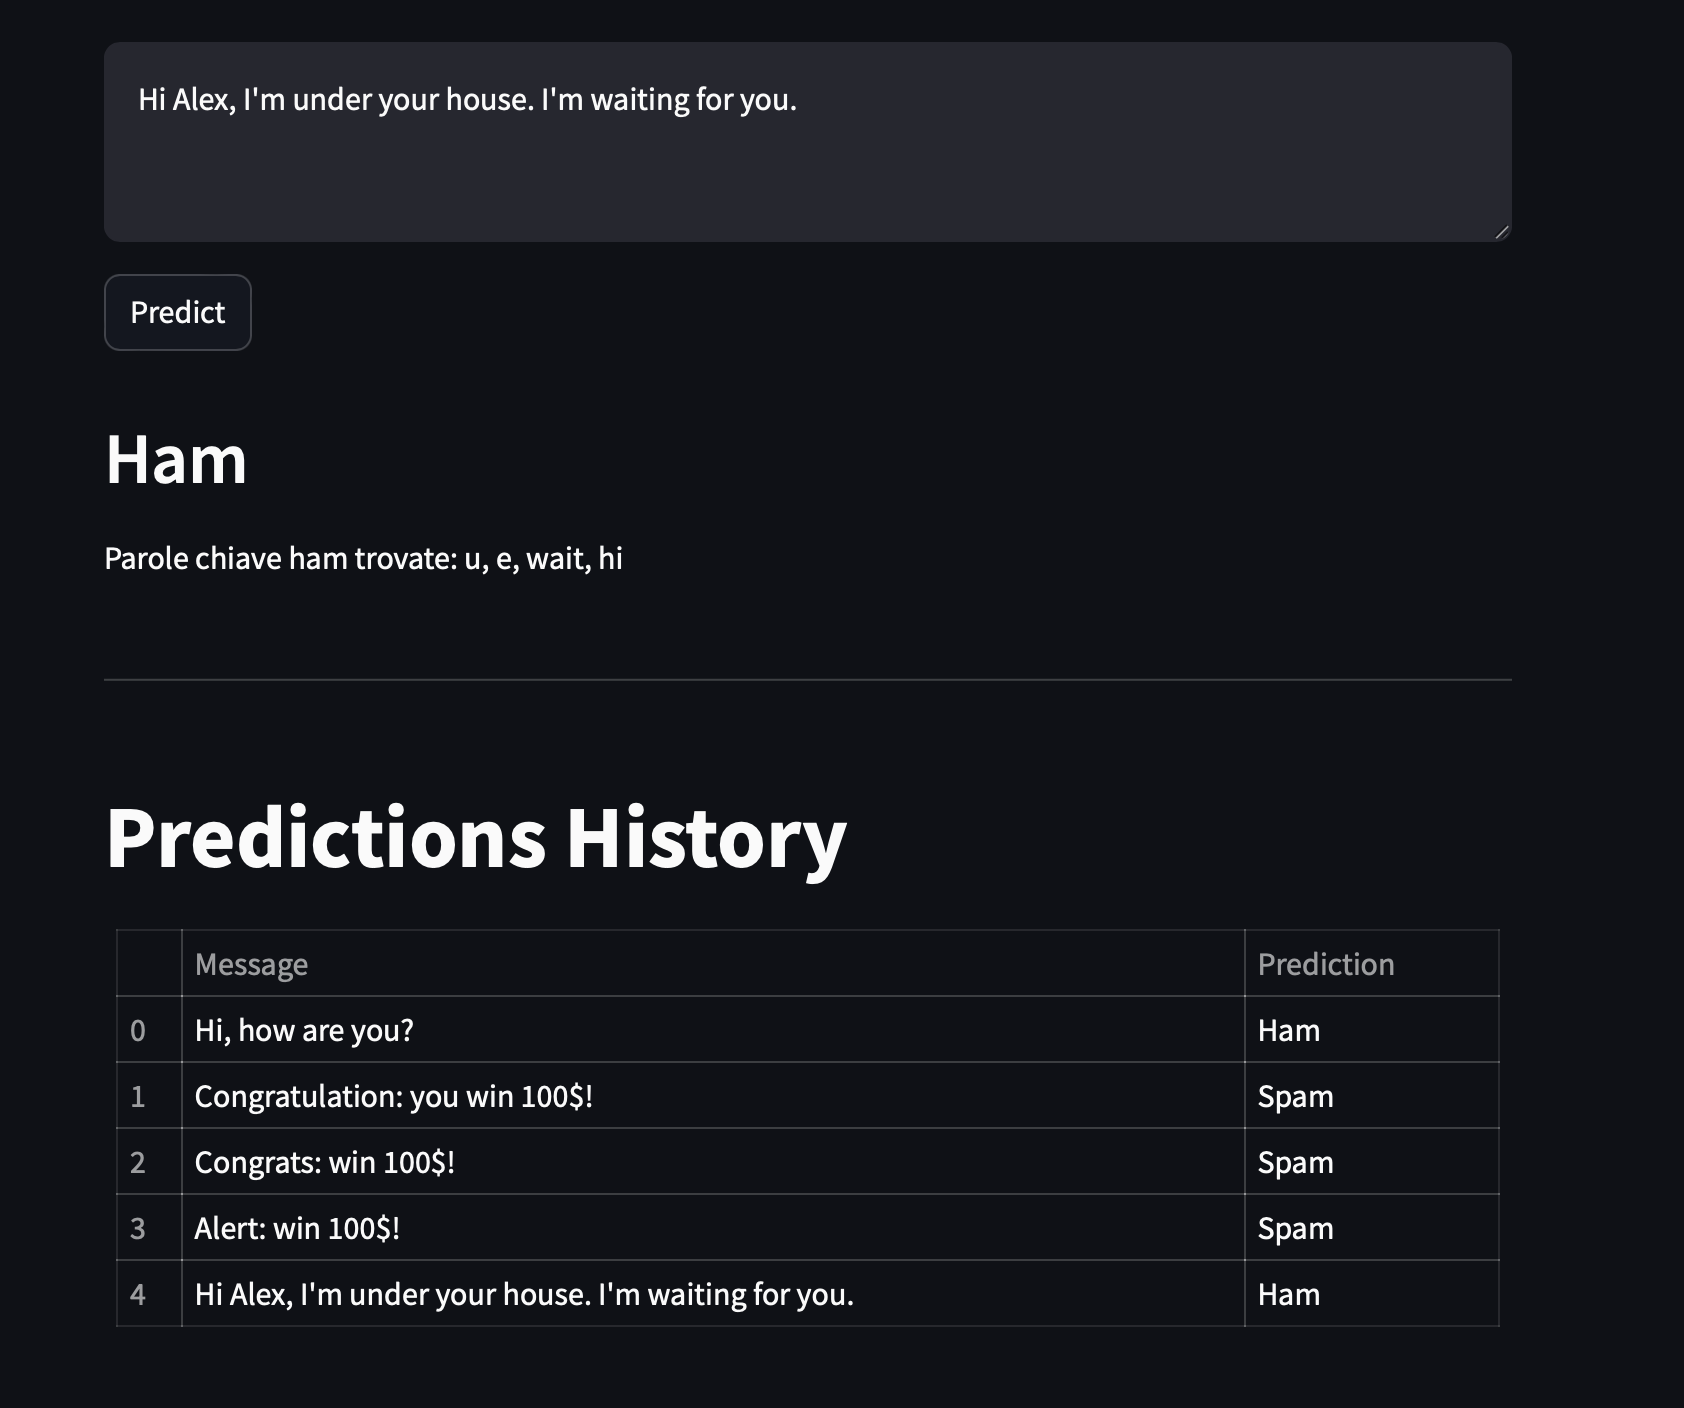
\includegraphics[width=1\linewidth]{images/app2.png}
                \caption{SMSecure app [explainability e history]}
                \label{fig:enter-label}
            \end{figure}

        \section{Conclusioni}
            Concludere il mio primo progetto di ML è stata un'esperienza ricca di apprendimento personale, in cui ho potuto affrontare nuove sfide, a partire dall'approfondimento del linguaggio Python fino ad arrivare a librerie più specifiche per il Machine Learning. L'utilizzo di algoritmi di classificazione e tecniche di preprocessing del testo sono state sfide interessanti e piacevoli. Per quanto riguarda gli obiettivi che mi ero proposto di realizzare ad inizio progetto posso dire di essere soddisfatto e di aver raggiunto ciò che mi ero prefissato.


\newpage
\bibliographystyle{alpha}
\bibliography{rif}


\end{document}